\documentclass[
	paper=a4,
	fontsize=11pt,
]{scrartcl}

% Sprache
\usepackage[%
%english,
ngerman
]{babel}
\usepackage[%
plain,
%english,
german
]{fancyref}
\usepackage{setspace}

\usepackage{bibgerm}

% preamble
%% $Id: settings.tex 20568 2010-09-10 14:56:08Z menski $

%%% === Textbody ==============================================================
\KOMAoptions{%
   DIV=11,% (Size of Text Body, higher values = greater textbody)
   % DIV=calc % (also areaset/classic/current/default/last) 
   % -> after setting of spacing necessary!   
   BCOR=5mm% (Bindekorrektur)
}%
%%% === Headings ==============================================================
\KOMAoptions{%
   %%%% headings
	% headings=small,  % Small Font Size, thin spacing above and below
   	% headings=normal, % Medium Font Size, medium spacing above and below
   	headings=big, % Big Font Size, large spacing above and below
   	%
   	%headings=noappendixprefix, % chapter in appendix as in body text
	%headings=nochapterprefix,  % no prefix at chapters
   	% headings=appendixprefix,   % inverse of 'noappendixprefix'
   	% headings=chapterprefix,    % inverse of 'nochapterprefix'
   	% headings=openany,   % Chapters start at any side
   	% headings=openleft,  % Chapters start at left side
   	%headings=openright, % Chapters start at right side      
   	%%% Add/Dont/Auto Dot behind section numbers 
   	%%% (see DUDEN as reference)
   	% numbers=autoenddot
   	% numbers=enddot
   	numbers=noenddot
   	% secnumdepth=3 % depth of sections numbering (???)
}   %
\setcounter{secnumdepth}{3}
%%% === Page Layout ===========================================================
\KOMAoptions{% (most options are for package typearea)
   % twoside=true, % two side layout (alternating margins, standard in books)
   twoside=false, % single side layout 
   % twoside=semi,  % two side layout (non alternating margins!)
   %
   twocolumn=false, % (true)
   %
   headinclude=false,%
   footinclude=false,%
   mpinclude=false,%      
   %
   headlines=2.1,%
	% headheight=2em,%
   headsepline=true,%
   footsepline=false,%
   cleardoublepage=empty %plain, headings
}%
%%% === Paragraph Separation ==================================================
\KOMAoptions{%
	% parskip=relative, % change indentation according to fontsize (recommanded)
   parskip=absolute, % do not change indentation according to fontsize
   parskip=false    % indentation of 1em
   % parskip=true   % parksip of 1 line - with free space in last line of 1em
   % parskip=full-  % parksip of 1 line - no adjustment
   % parskip=full+  % parksip of 1 line - with free space in last line of 1/4
   % parskip=full*  % parksip of 1 line - with free space in last line of 1/3
   % parskip=half   % parksip of 1/2 line - with free space in last line of 1em
   % parskip=half-  % parksip of 1/2 line - no adjustment
   % parskip=half+  % parksip of 1/2 line - with free space in last line of 1/3
   % parskip=half*  % parksip of 1/2 line - with free space in last line of 1em
}%
%%% === Table of Contents =====================================================
\setcounter{tocdepth}{3} % Depth of TOC Display
\KOMAoptions{%
   %%% Setting of 'Style' and 'Content' of TOC
   % toc=left, %
   toc=indented,%
   %
   toc=bib,
   % toc=nobib,
   % toc=bibnumbered,
   %
	% toc=index,%
   toc=noindex,
   %
   % toc=listof,
   toc=nolistof
   % toc=listofnumbered,
   %   
}%  
%%% === Lists of figures, tables etc. =========================================
\KOMAoptions{%
   %%% Setting of 'Style' and 'Content' of Lists 
   %%% (figures, tables etc)
	% --- General List Style ---
   listof=left, % tabular styles
   listof=indented, % hierarchical style
   % --- chapter highlighting ---
   % listof=chapterentry, % ??? Chapter starts are marked in figure/table
   % listof=chaptergapline, % New chapter starts are marked by a gap 
      		  			   	 % of a single line
   %listof=chaptergapsmall, % New chapter starts are marked by a gap 
   	    					   % of a smallsingle line
   % listof=nochaptergap, % No Gap between chapters
   %
   % listof=leveldown, % lists are moved one level down ???
   % --- Appearance of Lists in TOC
   % listof=notoc, % Lists are not part of the TOC
   listof=totoc % add Lists to TOC without number
   % listof=totocnumbered, % add Lists to TOC with number
}%  
%%% === Bibliography ==========================================================
%% Setting of 'Style' and 'Content' of Bibliography
\KOMAoptions{%
	% bibliography=oldstyle,%
   bibliography=openstyle,%
   % bibliography=nottotoc, % Bibliography is not part of the TOC
   % bibliography=totocnumbered, % add Bibliography to TOC with number
   bibliography=totoc % add Bibliography to TOC without number
}%
%%% === Index =================================================================
%% Setting of 'Style' and 'Content' of Index in TOC
\KOMAoptions{%
   index=nottotoc % index is not part of the TOC
	% index=totoc, % add index to TOC without number
}%
%%% === Titlepage =============================================================
\KOMAoptions{%
   titlepage=true %
   %titlepage=false %
}%
%%% === Miscellaneous =========================================================
\KOMAoptions{% 	
   footnotes=multiple% nomultiple
   %open=any,%
   %open=left,%
   %open=right,%
   %chapterprefix=false,%
   %appendixprefix=false,%
   %chapteratlists=10pt,% entry
}%
%% $Id: preamble.tex 20694 2010-09-21 18:47:18Z menski $

%% $Id: preamble-commands.tex 20694 2010-09-21 18:47:18Z menski $

\usepackage{xspace}
\usepackage{ifthen}
\usepackage{ifpdf}

\makeatletter

\providecommand{\IfPackageLoaded}[2]{\@ifpackageloaded{#1}{#2}{}}
\providecommand{\IfPackageNotLoaded}[2]{\@ifpackageloaded{#1}{}{#2}}
\providecommand{\IfElsePackageLoaded}[3]{\@ifpackageloaded{#1}{#2}{#3}}

\def \mail {}
\newcommand{\email}[1]{\def \mail {#1}}

\@ifundefined{frontmatter}{%
   \newcommand{\frontmatter}{%
      %In Roemischen Buchstaben nummerieren (i, ii, iii)
      \pagenumbering{roman}
   }
}{}
\@ifundefined{mainmatter}{%
   % scrpage2 benoetigt den folgenden switch
   % wenn \mainmatter definiert ist.
   \newif\if@mainmatter\@mainmattertrue
   \newcommand{\mainmatter}{%
      % -- Seitennummerierung auf Arabische Zahlen zuruecksetzen (1,2,3)
      \pagestyle{fancy}%%
      \pagenumbering{arabic}%%
   }
}{}
\@ifundefined{backmatter}{%
   \newcommand{\backmatter}{
      %In Roemischen Buchstaben nummerieren (i, ii, iii)
      \pagenumbering{Roman}
   }
}{}

% \def\thickhrulefill{\leavevmode \leaders \hrule height 1pt\hfill \kern \z@}
% \renewcommand{\maketitle}{\begin{titlepage}%
%     \let\footnotesize\small
%     \let\footnoterule\relax
    % \parindent \z@
    % \reset@font
    % \null
    % \vskip 10\p@
    % \hbox{\mbox{%
    %     \hspace{4pt}%
      %   		
\includegraphics[width=7em]{images/uni-logo}%
      %   \hspace{4pt}
      %   }%
      % \vrule depth 0.80\textheight%
      % \mbox{\hspace{2em}}
      % \vtop{% %%%%%%%%%%%%%%%%%%
      %   \vskip 20\p@
        % \begin{flushleft}
        %   \Huge \bfseries \@title \par
        % \end{flushleft}
        % \vskip 60\p@
        % \begin{flushleft}
        %   \LARGE BACHELORARBEIT \par 
        %   \vskip 5\p@
        %   \large zur Erlangung des akademischen Grades\\\Large\textit{Bachelor of Science}\\\large im Studiengang Informatik \par
        %   \vskip 5\p@
        %   \LARGE \@author \par
        %   \vskip 1\p@
        %   \large \mail \par
        % \end{flushleft}
	% 	\vskip 90\p@
        % \begin{flushleft}
        %   \large \@publishers \par
        % \end{flushleft}
        % \vskip 30\p@
        % \begin{flushleft}
        %   \large \@date \par
    %     \end{flushleft}
    %     \vfil
    %     }}        
    % \null
%   \end{titlepage}%
%   \setcounter{footnote}{0}%
% }

%\def\thickhrulefill{\leavevmode \leaders \hrule height 1pt\hfill \kern \z@}
%\renewcommand{\maketitle}{\begin{titlepage}%
%    \let\footnotesize\small
%    \let\footnoterule\relax
%    \parindent \z@
%    \reset@font
%    \null
%    \vskip 10\p@
%    \hbox{\mbox{%
%        \hspace{4pt}%
%			
\includegraphics[width=7em]{images/uni-logo}%
%        \hspace{4pt}
%        }%
%      \vrule depth 0.80\textheight%
%      \mbox{\hspace{2em}}
%      \vtop{% %%%%%%%%%%%%%%%%%%
%        \vskip 20\p@
%        \begin{flushleft}
%          \Huge \bfseries \@title \par
%          \LARGE \bfseries \@subtitle \par
%        \end{flushleft}
%        \vskip 60\p@
%        \begin{flushleft}
%          \LARGE Bachelor Thesis \par 
%          \vskip 5\p@
%          \large by \par
%          \vskip 5\p@
%          \LARGE \@author \par
%          \vskip 1\p@
%          \large \mail \par
%        \end{flushleft}
%		\vskip 120\p@
%        \begin{flushleft}
%          \large \@publishers \par
%        \end{flushleft}
%        \vskip 30\p@
%        \begin{flushleft}
%          \large \@date \par
%        \end{flushleft}
%        \vfil
%        }}        
%    \null
%  \end{titlepage}%
%  \setcounter{footnote}{0}%
%}

\makeatother

% Encoding
\usepackage[T1]{fontenc}
\usepackage[%
%	latin1,
	utf8
]{inputenc}

% Layout
\usepackage{fancyhdr}

% Refernces
\usepackage[]{prettyref}
%\newrefformat{cha}{Kapitel \ref{#1}}
%\newrefformat{sec}{Abschnitt \ref{#1}}
%\newrefformat{tab}{Tabelle \ref{#1} auf Seite \pageref{#1}}
%\newrefformat{fig}{Abbildung \ref{#1} auf Seite \pageref{#1}}
%\newrefformat{fig}{Abbildung \ref{#1}}
\newrefformat{fig}{Figure \ref{#1}}
%\newrefformat{lst}{Listing \ref{#1} auf Seite \pageref{#1}}

\usepackage{todonotes}

% Grafik
% \usepackage[%
% 	table
% ]{xcolor}
\usepackage{graphicx}
\usepackage{epstopdf}

% Mathe
\usepackage[%
	centertags,
	sumlimits,
	intlimits,
	namelimits,
	fleqn
]{amsmath}
\usepackage[
	all,
	warning
]{onlyamsmath}
\usepackage{fixmath}

\usepackage{tikz}
\usetikzlibrary{arrows}

% Berechnungen
\usepackage{calc}

% Textauszeichnung
\usepackage{soul}
\usepackage[normalem]{ulem}
\usepackage{url}
\usepackage[%
	babel,
	german=quotes,
	english=british
]{csquotes}
\usepackage{ragged2e}
\usepackage{multicol}
\usepackage[
	colorlinks=false,
	pdfborder={0 0 0},
]{hyperref}

% Floats
\usepackage{float}
\usepackage{flafter}
\usepackage[%
	section,
	above
]{placeins}
\usepackage[lofdepth=2]{subfig}
\usepackage{wrapfig}
\setlength{\intextsep}{0.5\baselineskip}

% Tabellen
\usepackage{booktabs}
\usepackage{multirow}
\usepackage{dcolumn}
\usepackage{ltxtable}

% Wissenschaft
\usepackage{units}

% Listings
%\usepackage{algorithmic}
%\usepackage{algorithm}
\usepackage[ruled,vlined,linesnumbered]{algorithm2e}
\usepackage{listings}
\lstset{ %
language=Java,                % choose the language of the code
basicstyle=\footnotesize,       % the size of the fonts that are used for the code
numbers=left,                   % where to put the line-numbers
numberstyle=\footnotesize,      % the size of the fonts that are used for the line-numbers
stepnumber=1,   	            % the step between two line-numbers. If it's 1 each line 
                                % will be numbered
numbersep=5pt,                  % how far the line-numbers are from the code
backgroundcolor=\color{white},  % choose the background color. You must add \usepackage{color}
showspaces=false,               % show spaces adding particular underscores
showstringspaces=false,         % underline spaces within strings
showtabs=false,                 % show tabs within strings adding particular underscores
%frame=single,	                % adds a frame around the code
tabsize=2,	                % sets default tabsize to 2 spaces
captionpos=b,                   % sets the caption-position to bottom
breaklines=true,                % sets automatic line breaking
breakatwhitespace=false,        % sets if automatic breaks should only happen at whitespace
%title=\lstname,                 % show the filename of files included with \lstinputlisting;
                                % also try caption instead of title
escapeinside={\%*}{*)},         % if you want to add a comment within your code
morekeywords={*,...}            % if you want to add more keywords to the set
}


%%% Local Variables: 
%%% mode: latex
%%% TeX-master: "../master"
%%% End: 

\usepackage[absolute]{textpos}

\newlength{\TitleLeft}
\newlength{\TitleRight}
\newlength{\TitleAbove}
\newlength{\TitleWidth}

\setlength{\TitleLeft}{2cm}
\setlength{\TitleRight}{2cm}
\setlength{\TitleAbove}{2cm}
\setlength{\TitleWidth}{\paperwidth-\TitleLeft-\TitleRight}

\newcommand{\BAUni}{Universität~Potsdam}
\newcommand{\BAInstitut}{Mathematisch-Naturwissenschaftliche~Fakultät\\Institut~für~Informatik}
\newcommand{\BABetreuerText}{Betreuer}
\newcommand{\BAAutor}{Sebastian~Menski (734272)\\menski@uni-potsdam.de}
\newcommand{\BATyp}{Seminararbeit\\Praktikum Paralleles Rechnen}
\newcommand{\BAAbschlussText}{}
\newcommand{\BAAbschluss}{}
\newcommand{\BATitle}{Einrichten eines Clusters zum Einspielen von Wikipedia-Traces}
\newcommand{\BABetreuer}{Prof. Dr. Bettina Schnor\\ & M.Sc. Jörg Zinke}
\newcommand{\BAOrt}{Potsdam}
\newcommand{\BAAbgabedatum}{26. Juli 2011}

\definecolor{uniblue}{rgb}{0.062745,0.17647,0.34118}

\renewcommand{\maketitle}{
  \thispagestyle{empty}
  \begin{textblock*}{\TitleWidth}(\TitleLeft,\TitleAbove)
    ~\hfill
\includegraphics[height=2.5cm]{images/uni-logo}\\[3mm]
    {\color{uniblue}\rule{\TitleWidth}{1mm}}\\[5mm]
    {
      \centering
      \sffamily\Large
      {\LARGE\BAUni}\\[0.5\baselineskip]
      {\large\BAInstitut}\\[4\baselineskip]
      {\BATyp}\\[\baselineskip]
      {\Huge\BATitle}\\[6\baselineskip]

%      {\BATyp}\\[7\baselineskip]
      
      \BAAutor\\[7\baselineskip]
      \begin{tabular}{rl}
         \BABetreuerText: & \BABetreuer
      \end{tabular}\\[3\baselineskip]
      \BAOrt, \BAAbgabedatum\par
    }
  \end{textblock*}
  ~\clearpage
}

%%% Local Variables: 
%%% mode: latex
%%% TeX-master: "../master"
%%% End: 


% macros
% % FancyRef
\newcommand*{\fancyrefalglabelprefix}{alg}
\newcommand*{\Frefalgname}{Algorithm}
\newcommand*{\frefalgname}{\MakeLowercase{\Frefalgname}}
\frefformat{main}{\fancyrefalglabelprefix}{%
  \textbf{\frefalgname\fancyrefdefaultspacing#1}#3}
\frefformat{vario}{\fancyrefalglabelprefix}{%
  \frefalgname\fancyrefdefaultspacing#1#3}
\frefformat{plain}{\fancyrefalglabelprefix}{%
  \frefalgname\fancyrefdefaultspacing#1}

% \newcommand{\marginnote}[1]{\marginpar{
% \raggedright\footnotesize
% \itshape#1\par}}
% \newcommand{\todo}[1]{\marginnote{\textbf{TODO:}#1}}

%%% Local Variables: 
%%% mode: latex
%%% TeX-master: "../master"
%%% End: 


\hypersetup{
  pdfauthor = {Sebastian Menski},
  pdftitle = {\BATitle},
}

\begin{document}
%% FRONTMATTER
\frontmatter
\maketitle
\clearpage

\tableofcontents
%\listoftodos
%% MAINMATTER
\clearpage
\mainmatter
\onehalfspacing
\section{Einleitung}
\label{sec:einleitung}

Um Webserver und Server Load Balancer zu testen werden verschiedenste Benchmarks verwendet. Oft nutzen diese Benchmarks synthetisch erzeugte Requests, im Falle von Webservern auch synthetische Websites. Dies hat zum Nachteil, dass kein realistisches Nutzerverhalten simuliert werden kann. Somit fehlt die Verbindung zu realistischen Lastsituationen. Zum Testen von existieren Webservern können realistische, aufgezeichnete Traces genutzt und modifiziert werden um realistischere Lasttests zu generieren. Für das Testen von Server Load Balancer bleibt weiterhin das Problem, dass auf existierende Benchmarks und Webanwendungen zurückgegriffen werden muss. 

Am Lehrstuhl Betriebssysteme und Verteilte Systeme von Frau Prof. Dr. Schnor
%, am Institut für Informatik der Universität Potsdam, 
schreibt M.Sc. Jörg Zinke seine Doktorarbeit zum Thema Server Load Balancing. Um die entwickelten Algorithmen anhand eines realistischen Benchmarks bzw. einer realistischen Webanwendung zu testen, soll die englische Wikipedia simuliert werden. Zum Testen stehen außerdem reale Webserver-Traces der Wikipedia zur Verfügung.

Als nächstes wird die Aufgabenstellung beschrieben. In Abschnitt \ref{sec:grundlagen} werden die nötigen Grundlagen für die Lösung der Aufgabe diskutiert und erläutert. Daraus ergibt sich das Konzept, welches in Abschnitt \ref{sec:konzept} vorgestellt wird. Dessen Implementation wird in Abschnitt \ref{sec:implementierung} erläutert. Die in Abschnitt \ref{sec:beispiel} präsentierten Daten, sollen die Zusammensetzung der Traces und die Wichtigkeit der Bild-Dateien, für das erfolgreiche Einspielen von Traces, verdeutlichen. Abschließend wird in Abschnitt \ref{sec:zusammenfassung} das Ergebnis dieser Arbeit zusammengefasst und in Abschnitt \ref{sec:ausblick} ein Ausblick auf die Weiterentwicklung der hier vorgestellten Lösung präsentiert.

\subsection{Aufgabenstellung}
\label{sec:aufgabestellung}

Ziel dieses Praktikums war es, eine Anwendung bzw. ein Skript zu entwickeln, welches es ermöglicht ein Webserver-Cluster mit einer Wikipedia-Umgebung einzurichten. Dazu wird ein gegebener Wikipedia-Dump genutzt und ein bestimmter Teil eines Wikipedia-Traces. Nach dem Einrichten sollen alle Server, die Artikel der englischen Wikipedia (entsprechende des Dumps) anbieten. Hinzu kommen die im benutzten Trace-Abschnitt verwendeten Bilddateien. Anschließend soll bei einem Wiedereinspielen des Trace-Abschnitts der Anteil der nicht gefundenen Ressourcen minimal sein. Daher ergeben sich folgende Unteraufgaben:
\begin{enumerate}
\item Filtern des Traces
\item Ermitteln und Bereitstellen der benötigten Ressourcen
\item Verteilen und Einrichten der präparierten Umgebung auf dem Cluster
\end{enumerate}

%%% Local Variables: 
%%% mode: latex
%%% TeX-master: "../master"
%%% End: 
\clearpage
\section{Grundlagen}
\label{sec:grundlagen}

Um eine Instanz der Wikipedia bereitzustellen benötigt man mehrere Komponenten. Als Basis benötigt man einen Webserver (empfohlen Apache httpd\footnote{\url{http://httpd.apache.org/}}), PHP (empfohlen $\geq$ 5.0) und MySQL (empfohlen $\geq$ 4.0). Als weitere Software wird Mediawiki\footnote{\url{http://www.mediawiki.org/}} benötigt, welches die Wikisoftware der Wikipedia ist. Nach der Installation dieser Komponenten ist ein leeres Wiki eingerichtet. Um daraus eine Instanz der Wikipedia zu machen, benötigt man eine Dump der Wikipedia. Ein Dump bezeichnet hier die Sicherung der Datenbanken der Mediawiki-Installation. Dabei ist zu beachten das jede Sprache in der Wikipedia, wiederum ein eigenes Wiki ist (z.B. \url{http://en.wikipedia.org/} oder \url{http://de.wikipedia.org/}). Somit benötigt man den Dump einer bestimmten Wikipedia, diese Dumps werden regelmäßig von der Wikimedia Foundation erstellt und zum Download angeboten\footnote{\url{http://dumps.wikimedia.org/}}. Leider enthalten diese Dumps wie bereits erwähnt nur die Sicherungen der Datenbanken und aus rechtlichen Gründen nicht die in den Wikipedia-Artikeln genutzten Bilder. Aber mit Hilfe eines Dumps und den vom Mediawiki bereitgestellten Skripten können zu mindestens die Wikipedia-Artikel in die Datenbank eingelesen werden.

\subsection{WikiBench}
\label{sec:wikibench}

Die für diese Arbeit genutzten Dumps und Traces stammen von der Internetseite \url{http://www.wikibench.eu/}. Bei WikiBench handelt es sich um ein Webanwendungs-Benchmark, welcher einen Dump der englischen Wikipedia und reale Traces der Wikipedia nutzt. WikiBench wurde im Laufe einer Abschlussarbeit \cite{wikibench} an der VU Universität Amsterdam entwickelt. Die genutzten Traces wurden zudem in dem Paper \cite{wikianal} analysiert.

Der Dump enthält über 6 Millionen Artikel der englischen Wikipedia. Die Traces enthalten 25.6 Milliarden HTTP-Requests in der Zeit vom 19. September 2007 bis zum 2. Januar 2008. Jeder Request besteht aus einer eindeutigen ID, einem Zeitstempel, einer URL und einem Feld, welches anzeigt ob es sich um eine Operation zum Speichern von Daten gehandelt hat (entweder \glqq{}save\grqq{} oder \glqq{}-\grqq{}). Beispiele (zur besseren Darstellung teilweise gekürzt):

\begin{small}
\begin{verbatim}
5399461277 1194892944.297 http://de.wikipedia.org/wiki/Potsdam -
5[...] 1194892392.420 http://en.wikipedia.org/w/index.php?[...]&action=submit save
\end{verbatim}
\end{small}



Die Requests sind vollständig anonymisiert und entsprechen nur 10\% der tatsächlichen Requests in diesem Zeitraum. Rund 43\% der Seitenanfragen richten sich an die englische Wikipedia, wobei insgesamt 32\% der Requests auf Bilder oder Thumbnails verweisen (vgl. \cite{wikianal}). Dieser Anteil zeigt, dass möglichst viele Bilder und Thumbnails bereitgestellt werden müssen, um ein sinnvolles Wiedereinspielen zu ermöglichen.

\subsection{Leistungsanalyse: Messen, Modellieren und Simulation}
\label{sec:mms}

In der Lehrveranstalltung \glqq{}Leistungsanalyse: Messen, Modellieren und Simulation\grqq{} (Sommersemester 2010) hatte Fabian Hahn, das Thema \glqq{}Server load balancing: Wikipedia\grqq{} \cite{mms}. Dabei war es seine Aufgabe den Server Load Balancer Perlbal mit Hilfe des Benchmarks httperf zu testen. Dazu nutzte er den Wikipedia-Dump und die Wikipedia-Traces von WikiBench. Die für diese Arbeit wichtigen Schlussfolgerungen aus seiner Arbeit waren, dass das Einspielen des Dumps sehr zeitintensiv und instabil ist, die Bilder nicht im Dump enthalten sind und nachgeladen werden müssen und die in den Wikipedia-Artikeln enthaltenen Thumbnails dynamisch generiert werden. Zum Nachladen der Bilder existiert im Internet ein Crawler\footnote{\url{http://meta.wikimedia.org/wiki/Wikix}}, welcher den Dump nach Bilderverweisen durchsucht und diese versucht herunterzuladen. Dabei ist zu beachten, dass er keine Thumbnails herunterlädt. Trotzdem ergibt sich das Problem, dass die Thumbnails direkt in den Traces aufgerufen werden und es nicht garantiert ist, dass der entsprechende Wikipedia-Artikel vorher im Trace-Verlauf enthalten ist. Somit müssten zu erst alle Thumbnails generiert werden, bevor der Trace eingespielt werden kann. Eine simple Strategie dafür wäre ein Aufruf aller enthaltenen Wikipedia-Artikel, was aber sequentiell nicht effektiv handhabbar ist.

\subsection{Erfahrungen Praktikum Paralleles Rechnen}
\label{sec:erfahrungen}

Zu Beginn des Praktikums lauteten die Aufgabenpunkte, für diese Arbeit:
\begin{enumerate}
\item Die Wikipedia Instanz sollte auf mehrere Server eines Clusters verteilt werden.
\item Die Server sollten durch einen Load Balancer verbunden werden.
\item Es sollte eine parallele Anwendung entwickelt werden, welche alle Wikipedia-Artikel aufruft.
\end{enumerate}
Durch dieses Vorgehen sollten alle nötigen Thumbnails für die Traces generiert werden. Nach dem erfolgreichen Aufsetzen aller Wikipedia-Instanzen und der Entwicklung einer parallelen Anwendung zum Abrufen der Wikipedia-Artikel, scheiterte diese Vorhaben jedoch an mehreren Faktoren. In erster Linie scheiterte es an der riesigen Datenmenge, welche durch die große Anzahl an Wikipedia-Artikel und Bildern erzeugt wurde. Die zu dieser Zeit genutzte Hardware stieß dabei an ihre Speichergrenzen. Hinzu kamen Probleme bei der Thumbnail-Generierung und Hardware-Defekte. Als Lösung des Speicherplatz-Problems bot sich an, nicht die gesamten Bilder und Thumbnails zu verwenden, sondern nur die benötigten Ressourcen für einen Abschnitt aus den Traces. Weiterhin bot es sich an gezielt die in diesem Trace-Abschnitt verwendeten Bilder und Thumbnails direkt von der aktuellen Wikipedia herunterzuladen. Durch diese neue Herangehensweise entstand die im Abschnitt \ref{sec:aufgabestellung} beschriebene Aufgabenstellung.

%%% Local Variables: 
%%% mode: latex
%%% TeX-master: "../master"
%%% End: 

\clearpage
\section{Konzept}
\label{sec:konzept}

Das Konzept der hier vorgestellten Lösung besteht aus 4 Teilschritten. Als Eingabe wird ein Trace, ein Zeitabschnitt und eine Liste an zu filternden URLs benötigt.

\begin{description}
\item[1. Analyse (optional):] Der erste Schritt ist optional und dient nur der Informationsgewinnung. Hierbei werden die Request des angegeben Traces nach Host-Adressen und Bild- bzw. Thumbnail-Vorkommen analysiert. Außerdem werden optional die Requests pro Sekunde grafisch dargestellt.
\item[2. Filterung:] Im zweiten Schritt, wird der gegeben Trace gefiltert. Dazu werden nur Requests weiterverarbeitet, die in dem angegeben Zeitabschnitt liegen. Außerdem werden nur Request beachtet bei denen das letzte Feld der Requestzeile (Speicherung von Daten; siehe \ref{sec:wikibench}) ein \glqq{}-\grqq{} enthält. Also keine Speicherung von Daten durchgeführt wurde. Da es sich sonst vermutlich um \texttt{POST} Request handelte, welche sich nicht zum Wiedereinspielen eignen, da der Request-Body fehlt. Abschließend werden nur die Requests gespeichert, welche den zu filternden URLs entsprechen. Damit können die Traces auf den existieren Dump angepasst werden. So werden in diesem konkreten Beispiel nur Requests auf die englische Wikipedia und die damit verbunden Bilder-Ressourcen gefiltert.
\item[3. Download:] In diesem Schritt wird nun der gefilterte Trace ausgewertet und enthaltene Request für Bilder oder Thumbnails verarbeitet. Dazu wird zuerst geprüft ob die entsprechende Ressource bereits in einem früheren Durchlauf heruntergeladen wurden, wenn nicht wird versucht sie herunterzuladen. Dazu wird die im Trace angegebene URL genutzt. Ist die Ressource unter dieser URL nicht mehr verfügbar wurde sie seit Erstellung des Traces, entweder verschoben bzw. umbenannt oder gelöscht. Leider ist es dann nicht möglich, diese Ressource lokal bereitzustellen. Nachdem alle verfügbaren Ressourcen heruntergeladen wurden, müssen die Bilder der Wikipedia Datenbank bekannt gemacht werden. Dafür existiert ein PHP Skript im Mediawiki, welches Metadaten der Bilder in der Datenbank abspeichert. Dieses Skript ist sehr langsam und speicherintensiv, allerdings existiert leider keine Alternative.
\item[4. Installation:] Nachdem alle Ressourcen heruntergeladen wurden und die Datenbank aktualisiert wurde, können diese auf die anderen Server im Cluster transferiert werden und dort lokal eingerichtet werden. Anschließend sind alle Server des Clusters mit der selben Wikipedia Instanz ausgestattet.
\end{description}
Bis auf Schritt 1 sind alle Schritte erforderlich und benötigen mindestens einen Durchlauf des vorherigen Schrittes. Das heißt Schritt 3 kann erst ausgeführt werden, wenn Schritt 2 mindestens einmal ausgeführt wurde. Dann kann Schritt 3 aber beliebig wiederholt werden, ohne das Schritt 2 noch einmal ausgeführt werden muss. Das gleiche gilt für Schritt 4 bezüglich Schritt 3.

Ein weitere Punkt des Konzepts ist es, alle Schritte in einer Anwendung zu vereinen und diese Anwendung über eine Konfigurationsdatei zu steuern. Die Verwendung von Kommandozeilenoptionen schien nicht ratsam auf Grund der Fülle an Einstellungsmöglichkeiten und benötigten Parametern. Des weiteren, sollte die verfügbare CPU möglichst effizient ausgenutzt werden, weshalb eine Parallelisierung der Anwendung sinnvoll ist.

%%% Local Variables: 
%%% mode: latex
%%% TeX-master: "../master"
%%% End: 

\clearpage
\section{Implementierung}
\label{sec:implementierung}

In diesem Abschnitt wird die Implementierung des in Abschnitt \ref{sec:konzept} vorgestellten Konzepts besprochen. Dazu werden als erstes die Voraussetzungen für das Ausführen der Anwendung und die Einrichtung der Server beschrieben (siehe Abschnitt \ref{sec:voraussetzungen}). Anschließend wird das Entwickelte Skript vorgestellt (siehe Abschnitt \ref{sec:setupskript}) und die dazu gehörige Konfigurations-Datei erläutert (siehe Abschnitt \ref{sec:konfigurationsdatei}). Zum Abschluss wird der Ablauf des Skripts erläutert (siehe Abschnitt \ref{sec:ablauf}).

\subsection{Voraussetzungen}
\label{sec:voraussetzungen}

Wie bereits teilweise in Abschnitt \ref{sec:grundlagen} beschrieben, benötigt man auf einem Webserver, der eine Wikipedia-Instanz bereitstellen soll, folgende Software:
\begin{itemize}
\item Webserver (empfohlen Apache httpd\footnote{\url{http://httpd.apache.org/}})
\item PHP (empfohlen $\geq$ 5.0)
\item MySQL (empfohlen $\geq$ 4.0)
\item ImageMagick (empfohlen zur Generierung von Thumbnails)
\end{itemize}

Außerdem wird auf dem Rechner, auf dem das Setup-Skript ausgeführt wird, mindestens Python 2.6 benötigt und gegebenenfalls \texttt{gnuplot}. Zudem muss ein Mediawiki\footnote{\url{http://www.mediawiki.org/}} installiert und der Wikipedia Dump in die Datenbank eingespielt sein. Auf den Servern, auf denen die Wikipedia Umgebung installiert werden soll, wird mindestens Python 2.4 benötigt.

In diesem konkreten Fall wurde die Mediawiki Version 1.16.5 genutzt und der Dump der Wikipedia Artikel zuerst mit dem Programm \texttt{xml2sql}\footnote{\url{http://meta.wikimedia.org/wiki/Xml2sql/}} in SQL transformiert und dann mit dem Programm \texttt{mysqlimport} in die Datenbank importiert. Dieses Verfahren wird offiziell nicht empfohlen, aber es stellte sich als schneller und sicherer heraus als die Nutzung des PHP Skripts vom Mediawiki.

Anschließend sollte die Datenbank in diesem Zustand gesichert werden, da dieser Stand der Datenbank wieder benötigt wird, falls ein anderer Abschnitt des Traces vorbereitet werden soll. Dazu sollte das MySQL Verzeichnis (z.B. \texttt{/var/lib/mysql/}) per \texttt{tar} gepackt werden und gegebenenfalls noch komprimiert werden per \texttt{gzip} oder \texttt{bzip2}. Dieses Archiv wird später bei der Konfiguration des Setup-Skripts benötigt.

Nach der Installation vom Mediawiki (der Ordner des Mediawiki sollte \glqq{}w/\grqq{} genannt werden) muss die Datei \texttt{LocalSettings.php} noch angepasst werden. Dazu sollten folgende Zeilen ergänzt werden:
\begin{verbatim}
$wgArticlePath      = '/wiki/$1';
$wgScriptPath       = "/w";

$wgMaxShellMemory   = "unlimited";
$wgMaxShellFileSize = "unlimited";

require_once( "$IP/extensions/Cite/Cite.php" );
require_once( "$IP/extensions/ImageMap/ImageMap.php" );
require_once( "$IP/extensions/OggHandler/OggHandler.php" );
require_once( "$IP/extensions/ParserFunctions/ParserFunctions.php" );
\end{verbatim}
Die angegeben Extensions müssen dann noch heruntergeladen werden und in dem \texttt{extensions} Ordner hinterlegt werden. Dies ist z.B. über das SVN-Repository\footnote{\url{http://svn.wikimedia.org/svnroot/mediawiki/tags/REL1_16_5/extensions/}} des Mediwiki möglich. Damit der Apache httpd Server mit den verschieden URL-Formen der Wikipedia zurecht kommt, sollte noch folgende Eintrag in der httpd-Konfigurationsdatei (welche z.B. unter  \texttt{/etc/httpd/conf/httpd.conf} zu finden ist) ergänzt werden (wobei der Pfad zur \texttt{index.php} anzupassen ist):
\begin{verbatim}
Alias /wiki "/var/www/html/w/index.php"
\end{verbatim}
Es gibt noch weitere Möglichkeiten die Unterstützung der Short-URLs von Wikipedia zu erreichen, diese sind in dem Mediawiki Wiki\footnote{\url{http://www.mediawiki.org/wiki/Manual:Short_URL}} nachzulesen.

Bei der Verwendung von RedHat basierten Systemen (wie z.B. CentOS) ist zu beachten, dass in dem Paket \texttt{gnome-vfs2} bis zur Version 2.16.2-8.el5 ein Bug\footnote{\url{http://rhn.redhat.com/errata/RHBA-2011-0441.html}} die korrekte Ausführung von ImageMagick verhindert. Dadurch konnten keine Thumbnails für SVG Dateien erstellt werden. Daher ist es empfehlenswerte mindestens die genannte Version des Pakets zu installieren.

\subsection{Setup-Skript}
\label{sec:setupskript}

Die entwickelte Anwendung ist ein Python 2.6 Skript \texttt{setup\_env.py} und nutzt das ebenfalls selbst entwickelte Modul \texttt{ppr}. Der Sourcecode liegt der Ausarbeitung bei oder kann aus einem GIT-Repository\footnote{\url{https://github.com/menski/ppr-s11}} heruntergeladen werden.

In Abbildung \ref{fig:classes} wird das Klassendiagramm des \texttt{ppr} Moduls gezeigt. Die Basisklasse \texttt{Process} erbt von der Klasse \texttt{multiprocessing.Process}. Daran ist zu erkennen das fast jede Klasse ebenfalls ein eigener Prozess ist. Somit können verschieden Aufgaben in dem Skript parallel durchgeführt werden. Die Kommunikation zwischen den Prozessen wird über sogenannte \texttt{Pipes} realisiert, wodurch Daten nicht lange im Speicher gehalten werden müssen.

\begin{figure}
  \centering
  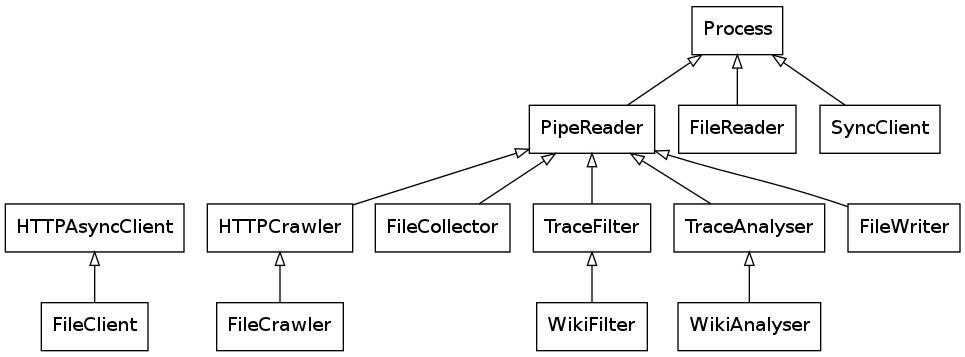
\includegraphics[width=\textwidth]{images/classes.png}
  \caption{Klassendiagramm des \texttt{ppr}-Moduls}
  \label{fig:classes}
\end{figure}

\subsubsection{Klassen}
\label{sec:klassen}

\begin{description}
\item[Process:] Basisklasse, welche von \texttt{multiprocessing.Process} erbt und eine Logger bereitstellt.
\item[SyncClient:] Ist eine Klasse, die genutzt wird um eine Wikipedia Instanz auf einen anderen Rechner zu kopieren.
\item[FileReader:] Diese Klasse liest eine Datei ein und sendet den Inhalt zur Verarbeitung an eine Menge von \texttt{Pipes}. Dabei ist es möglich die Funktion zum Öffnen der Datei anzugeben, um z.B. komprimierte Dateien zu öffnen.
\item[PipeReader:] Eine Klasse, welche eine \texttt{Pipe} nach Außen anbietet, über die sie mit Daten versorgt werden kann.
\item[FileWriter:] Erbt von der Klasse \texttt{PipeReader} und speichert die übergeben Daten in einer Datei. Wiederum ist es möglich eine Funktion zum Öffnen der Datei anzugeben, um z.B. komprimierten Dateien zu schreiben.
\item[TraceAnalyser/WikiAnalyser:] Spezielle \texttt{PipeReader} zur Analyse von Traces und zum Erstellen von Statistiken und Grafiken.
\item[TraceFilter/WikiFilter:] Klassen zum Filtern von Traces, welche ebenfalls von \texttt{PipeReader} erben.
\item[HTTPAsyncClient/FileClient:] Klassen, welche das Python Modul \texttt{asynchat} nutzen um HTTP1.1 Requests zu versenden. Die Klasse \texttt{FileClient} kann außerdem den Response in einer Datei speichern.
\item[HTTPCrawler/FileCrawler:] Klassen, die unter Nutzung der \texttt{HTTPAsyncClient/FileClient} Klassen und dem Python Modul \texttt{asyncore}, asynchrone HTTP Request versenden.
\item[FileCollector:] Eine Unterklasse von \texttt{PipeReader}, welche überprüft ob eine Datei bereits im Dateisystem existiert und falls nicht diese mit Hilfe der \texttt{FileCrawler} Klasse versucht herunterzuladen.
\end{description}

\subsubsection{Konfigurations-Datei}
\label{sec:konfigurationsdatei}

Ein vollständige Konfigurations-Datei ist im Anhang \ref{sec:konfiguration} aufgeführt. In diesem Abschnitt sollen die einzelnen Bereiche der Konfigurations-Datei erläutert werden.

\paragraph{[general]}

In dem \texttt{general} Abschnitt können die einzelnen Schritte des Skritps aktiviert bzw. deaktiviert werden (siehe dazu Abschnitt \ref{sec:konzept}). Außerdem kann das Log-Level gewählt werden und festgelegt werden ob bei der Analyse eine Grafik für die Requests pro Sekunde erstellt werden soll (dazu ist \texttt{gnuplot} nötig).

\paragraph{[trace]}

Der folgende \texttt{trace} Abschnitt gibt den Pfad zur Trace-Datei an und ob sie mit \texttt{gzip} komprimiert ist.

\paragraph{[filter]}

Im \texttt{filter} Abschnitt wird das Zeitintervall definiert, nach dem der Trace gefiltert wird. Dabei wird das Format $a:b$ genutzt und auf die folgende Weise interpretiert: $a$ ist ein UNIX-Zeitstempel, wenn $a > b$ gilt wird $b$ als Anzahl von Sekunden interpretiert und auf $a$ addiert, sonst wird $b$ ebenfalls als UNIX-Zeitstempel interpretiert. Als nächstes wird eine Hostname bestimmt, der genutzt wird um einen modifizierten Trace zu erstellen, welcher später zum Wiedereinspielen genutzt werden kann. Um nach bestimmten URLs zu filtern kann ein regulärer Ausdruck angegeben werden. Abschließend kann bestimmt werden, ob die gefilterten Traces mit \texttt{gzip} komprimiert gespeichert werden.

\paragraph{[download]}

Der \texttt{download} Abschnitt definiert das Verhalten beim Herunterladen von Bilder. Dazu wird ein Pfad angegeben, an dem nach bereits heruntergeladen Bilder gesucht wird und ebenfalls die neue heruntergeladenen Bilder gespeichert werden. Weiterhin kann der Port angegeben werden, über den die Requests versendet werden, um neue Bilder herunterzuladen. Die \texttt{async} Option gibt die parallel aufgebauten, asynchronen Verbindungen an. Des weiteren, werden die Pfade zu der Mediawiki- und MySQL-Installation, sowie der Name des lokal laufenden MySQL-Services benötigt. Mit den Optionen \texttt{clean\_images} und \texttt{clean\_mysql} kann bestimmt werden ob die aktuell in der Mediawiki-Installation vorhanden Bilder anfangs gelöscht werden sollen, bzw. ob die Datenbank vor dem einlesen der Bilder gelöscht werden soll und durch eine \glqq{}saubere\grqq{} Datenbank ersetzt werden soll. Diese \glqq{}saubere\grqq{} Datenbank wird über die Option \texttt{mysql\_archive} bestimmt. Die nach dem erfolgreichen Einrichten gepackten Mediawiki- und MySQL-Archive werden an dem Pfad gespeichert, der mit der Option \texttt{output\_dir} bestimmt wird.

\paragraph{[install]}

Der \texttt{install} Abschnitt ist der letzte notwendige Abschnitt. Er besteht allein aus einem String, welcher die Server angibt auf denen die Wikipedia-Instanz installiert werden soll und die dafür zu verwendende Konfiguration. Dabei ist der String eine durch \glqq{}:\grqq{} getrennte Liste. Jedes Element besteht aus einem Konfigurations-Namen, welcher durch ein \glqq{}@\grqq{} von einer einer Liste (getrennt durch Kommata) von IP-Adressen oder Hostname getrennt ist. Für jeden angegebenen Konfigurations-Namen muss wiederum ein Abschnitt in der Konfigurations-Datei angelegt werden. Diese Abschnitte bestehen dann aus dem Usernamen auf dem Server, dem Verzeichnis in, das die zu übertragenden Daten kopiert werden, dem Verzeichnis in dem das Mediawiki bzw. die MySQL-Datenbank installiert werden soll und dem Namen des MySQL-Service auf dem Server.

\subsubsection{Ablauf}
\label{sec:ablauf}
In diesem Abschnitt soll der Ablauf des Skripts dargestellt werden und beschrieben werden, welche Dateien erstellt werden.

\begin{enumerate}
\item Die Konfigurations-Datei wird eingelesen und auf Korrektheit geprüft.
\item Sofern der Analyse-Schritt oder Filter-Schritt aktiviert wurde, wird ein \texttt{FileReader} für das Tracefile erzeugt. Ist eine Analyse gefordert wird ein \texttt{WikiAnalyser} erzeugt bzw. ist die Filterung gefordert ein \texttt{WikiFilter}. Der \texttt{FileReader} sendet nun die gelesen Daten an die erzeugten Instanzen. Wurde eine \texttt{WikiAnalyser} erzeugt, erstellt dieser für eine Trace-Datei \texttt{trace.gz}, die folgenden Dateien:
  \begin{itemize}
  \item \texttt{trace.gz.stats} (Statistiken zum Trace)
  \item \texttt{trace.image.gz} (Alle Requests, die ein Bild anfordern)
  \item \texttt{trace.thumb.gz} (Alle Requests, die ein Thumbnail anfordern)
  \item \texttt{trace.page.gz} (Alle restlichen Requests)
  \item \texttt{trace.gz.eps} und \texttt{trace.gz.log} (falls die \texttt{plot} Option aktiviert wurde; Requests pro Sekunde Graph und gnuplot Ausgabe)
  \end{itemize}
Eine \texttt{WikiFilter} Instanz erzeugt die Dateien \texttt{trace.timestampA-timestampB.gz} (gefilterter Trace) sowie \texttt{trace.timestampA-timestampB.rewrite.gz} (Trace zum Wiedereinspielen). Außerdem erzeugt sie eine \texttt{WikiAnalyser} Instanz, womit ebenfalls für den gefilterten Trace, die oben beschrieben Datei erzeugt werden.
\item Im nächsten Schritt wird, sofern gewünscht, zuerst das Bilder-Verzeichnis von der Mediawiki-Installation geleert. Dann wird jeweils ein \texttt{FileReader} und ein \texttt{File\-Collector} für die benötigten Bilder bzw. Thumbnails erzeugt. Nachdem der Download abgeschlossen ist wird die Mediawiki-Installation gepackt und parallel die Bilder in die MySQL-Datenbank eingelesen und die MySQL-Datenbank ebenfalls gepackt.
\item Im letzten Schritt wird nun für jeden Server auf dem die Wikipedia-Instanz eingespielt werden soll, ein \texttt{SyncClient} erzeugt, der die gepackte MediaWiki-Installation, die gepackte MySQL-Datenbank und die Datei \texttt{ppr/server.py}, mittels \texttt{scp}, auf den entsprechenden Server kopiert. Und anschließend die kopierte Datei \texttt{server.py} mit entsprechenden Parametern über \texttt{ssh} aufruft. Das \texttt{server.py} Skript, welches wie bereits erwähnt Python 2.4 benötigt, entpackt die kopierten Archive auf dem Server und richtet die Umgebung ein. Anschließend ist auf dem Server die gewünschte Wikipedia-Instanz eingerichtet.
\end{enumerate}

\section{Beispiel: Trace-Analyse und -Filterung}
\label{sec:beispiel}

Die Trace-Analyse und -Filterung soll in diesem Kapitel anhand eines Beispiel Traces gezeigt werden. Dazu wurde die Trace-Datei \texttt{wiki.1194899823.gz}\footnote{\url{http://www.wikibench.eu/wiki/2007-11/wiki.1194899823.gz}} gewählt. Die Analyse dieses Traces ergibt die in Tabelle \ref{tab:trace-full} dargestellten Werte und der Verlauf der Requests pro Sekunde wird in Abbildung \ref{fig:trace-full} gezeigten. Filtert man diesen Trace nun für das Intervall 1194892290-1194894090 und nach den englischen Artikeln, erhält meinen einen Trace der durch die Tabelle \ref{tab:trace-filtered} und die Abbildung \ref{fig:trace-filtered} beschrieben wird. Es ist zu erkennen das der größte Teil der Requests Medien-Dateien abruft, welche über den Host \texttt{upload.wikimedia.org} erreichbar sind. Bei dem Abruf von Wikipedia Artikeln dominiert klar die englische Wikipedia und die Requests, welche mit \glqq{}save\grqq{} gekennzeichnet sind, können vernachlässigt werden.

\begin{table}
  \centering
  \begin{tabular}{|rr|}\hline
    \textbf{General} & \\\hline
    tracefile: & wiki.1194899823.gz \\
    start time: & Mon, 12 Nov 2007 18:31:30 +0000 \\
    end time: & Mon, 12 Nov 2007 19:31:35 +0000 \\
    duration: & 3604.986 sec \\
    lines: & 17.518.902 \\
    requests: & 17.518.817 \\
    page requests: & 7969566 (45,5\%) \\
    media requests: & 9.549.251 (54,5\%) \\
    errors: & 85 \\
    save operations: & 3.309 (0,02\%)\\\hline\hline
    \textbf{Hosts} & \\\hline
    upload.wikimedia.org: & 9.549.251 (54,5\%) \\
    en.wikipedia.org:&  3.228.167 (18,4\%) \\
    meta.wikimedia.org: &  977.302 (5,6\%) \\
    de.wikipedia.org:  & 747.068 (4,2\%)\\\hline
  \end{tabular}
  \caption{Trace-Analyse der Datei \texttt{wiki.1194899823.gz}}
  \label{tab:trace-full}
\end{table}

\begin{figure}
  \centering
  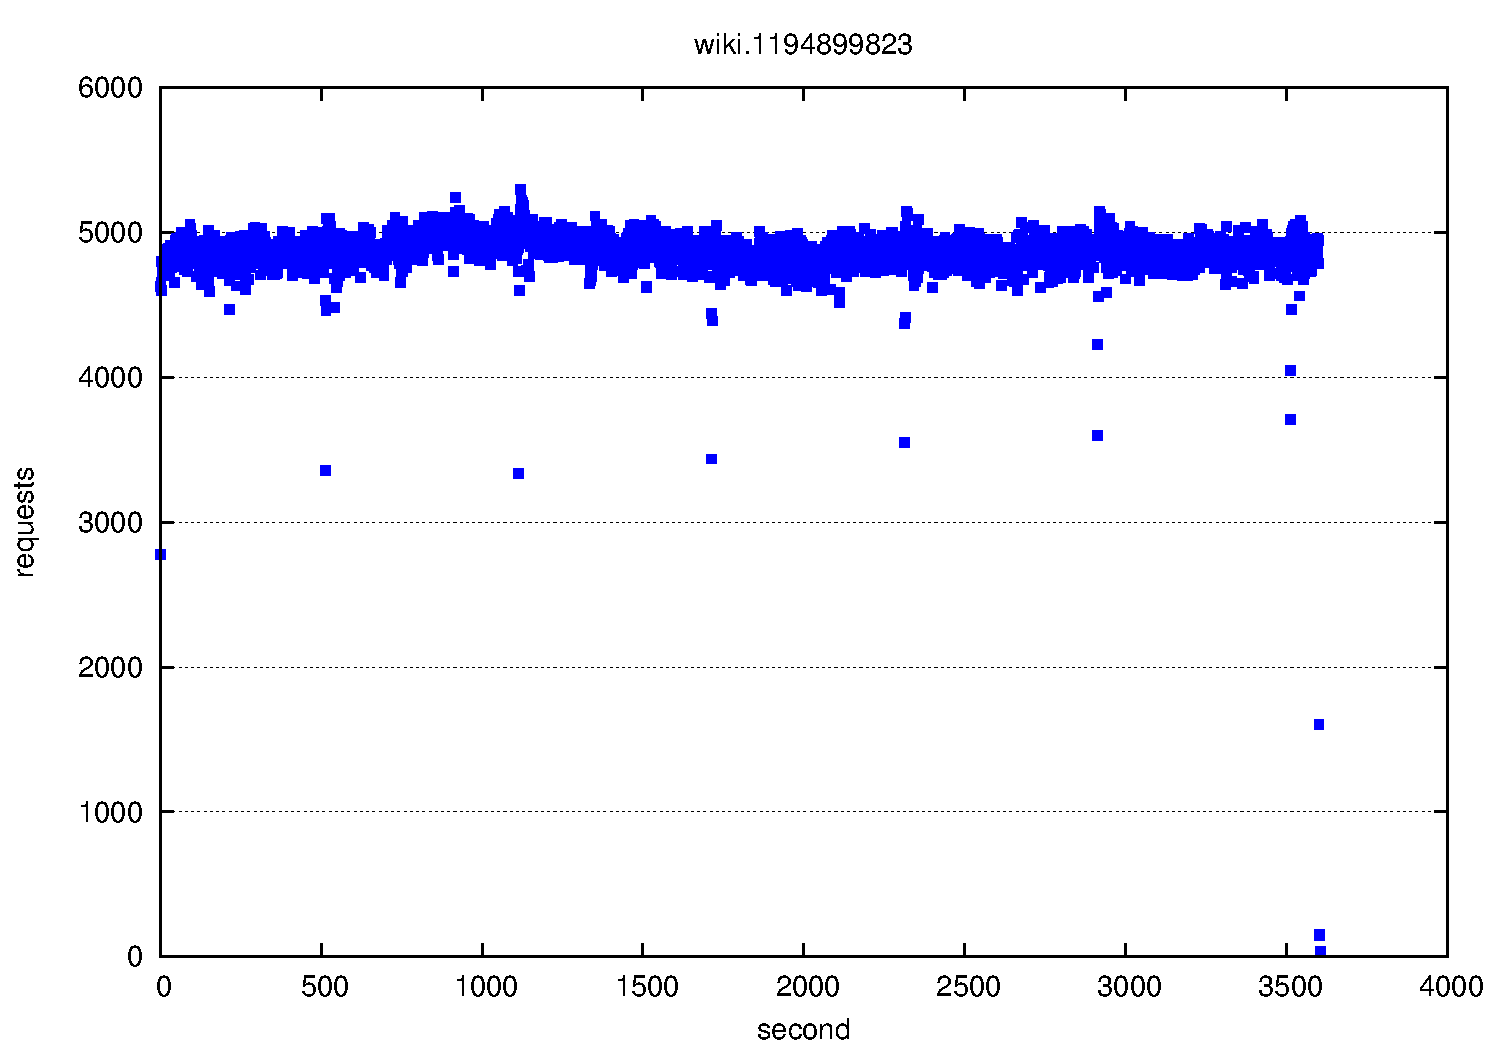
\includegraphics[width=\textwidth]{images/trace-full}
  \caption{Requests pro Sekunde der Datei \texttt{wiki.1194899823.gz}}
  \label{fig:trace-full}
\end{figure}

\begin{table}
  \centering
  \begin{tabular}{|rr|}\hline
    \textbf{General} & \\\hline
    tracefile: & wiki.1194899823.1194892290-1194894090.gz\\
    start time: & Mon, 12 Nov 2007 18:31:30 +0000\\
    end time: & Mon, 12 Nov 2007 19:01:30 +0000\\
    duration: & 1800.788 sec\\
    lines: & 4795845\\
    requests: & 4.795.845\\
    page requests: & 1.599.427 (33,3\%) \\
    media requests: & 3.196.418 (66,6\%) \\
    errors: & 0\\\hline\hline
    \textbf{Hosts} & \\\hline
    upload.wikimedia.org: & 3.196.418 (66,6\%) \\
    en.wikipedia.org: & 1.599.427 (33,3\%) \\\hline
  \end{tabular}
  \caption{Trace-Analyse der Datei \texttt{wiki.1194892290-1194894090.1194899823.gz}}
  \label{tab:trace-filtered}
\end{table}

\begin{figure}
  \centering
  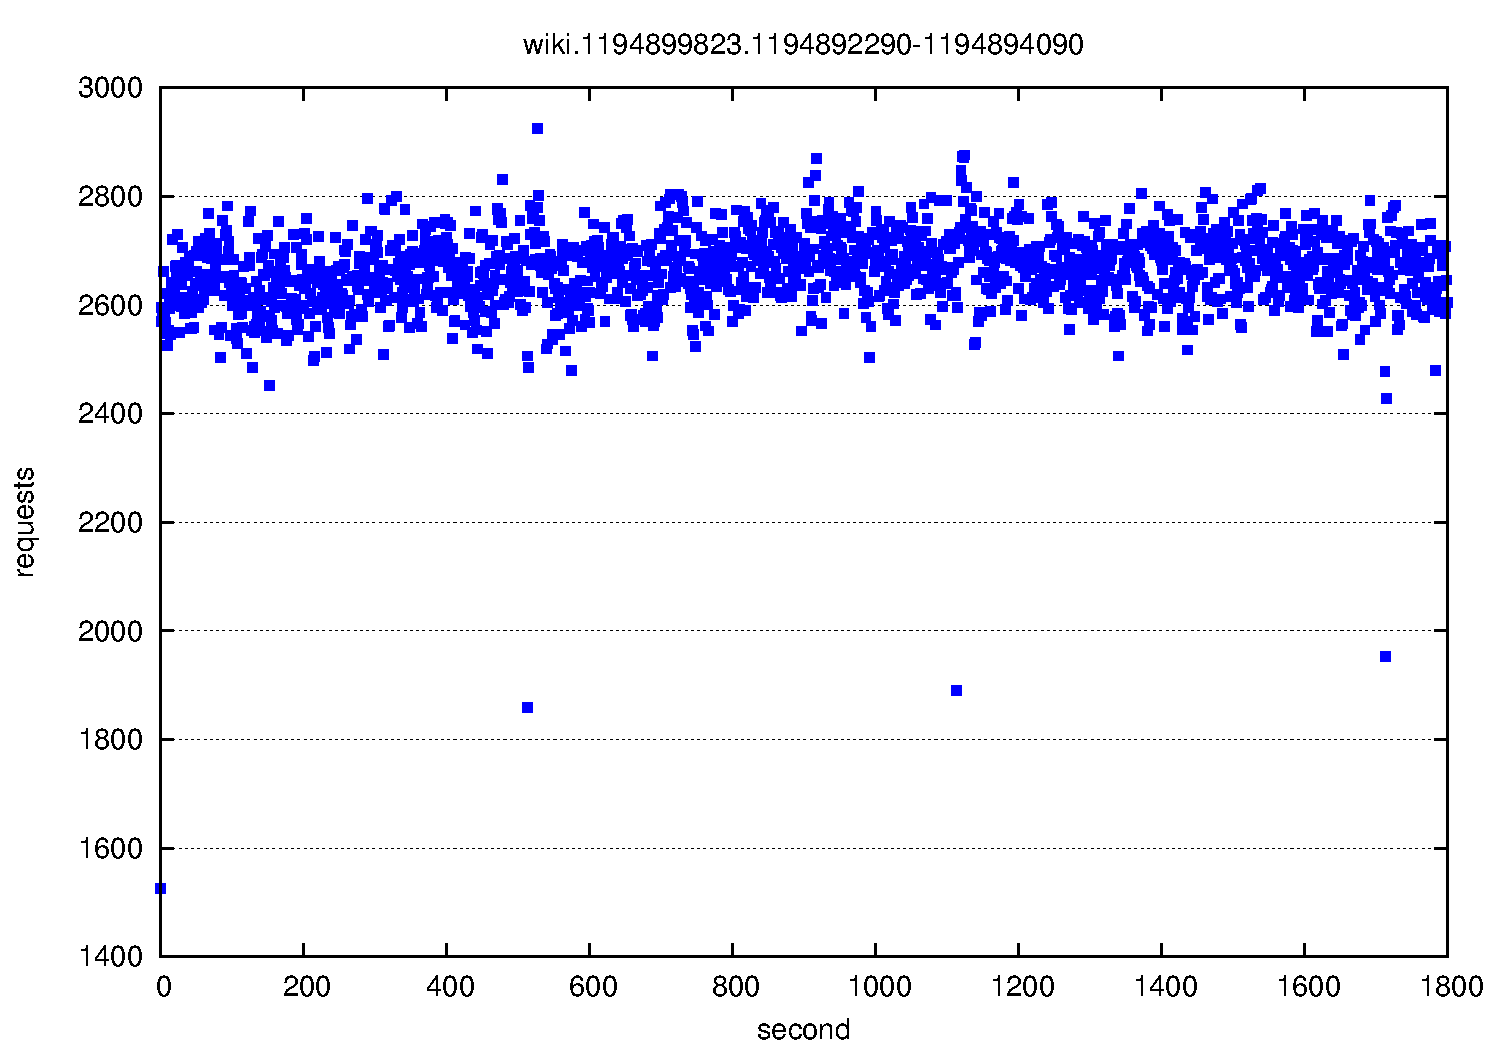
\includegraphics[width=\textwidth]{images/trace-filtered}
  \caption{Requests pro Sekunde der Datei \texttt{wiki.1194892290-1194894090.1194899823.gz}}
  \label{fig:trace-filtered}
\end{figure}

%%% Local Variables: 
%%% mode: latex
%%% TeX-master: "../master"
%%% End: 

\clearpage
\section{Zusammenfassung}
\label{sec:zusammenfassung}

Das in dieser Arbeit vorgestellt Skript ermöglicht es eine lokale Installation der Wikipedia mit Bildern anzureichern. Außerdem kann die lokale Installation anschließend auf weitere Server übertragen und dort eingerichtet werden. Damit ist die in Abschnitt \ref{sec:aufgabestellung} beschriebene Aufgabenstellung erfüllt. Das Skript ermöglicht durch die Parallelisierung anhand von Prozessen, eine optimale Auslastung der zu Verfügung stehenden Rechenleistung. Außerdem ist das Skript durch die parallel Abarbeitung sehr Speicher schonend, was sich besonders bei großen Traces auszahlt. Trotzdem ist die Ausführung des Skripts mit allen Schritten immer noch sehr zeitintensiv. Was an den großen Datenmengen liegt, welche verarbeitet, kopiert und verschoben werden müssen. 

Zur Stabilität des Skriptes kann keine klare Aussage getroffen werden. Aufgrund einer sehr kurzen Entwicklungszeit und mehrerer Hardwaredefekte konnte es kaum auf dem Produktiv-System getestet werden. Allerdings konnten mit Hilfe des Skriptes 4 Server, für ein 30 minütigen Trace-Ausschnitt, erfolgreich eingerichtet werden. Es liegen jedoch keine Messungen vor, wie hoch der aktuelle Anteil von nicht erreichbaren Ressourcen ist.

\section{Ausblick}
\label{sec:ausblick}

Wie bereits in der Zusammenfassung (siehe Abschnitt \ref{sec:zusammenfassung}) erwähnt, konnte das Skript kaum getestet werden. Hier bedarf es weitere Praxis-Tests und gegebenenfalls Fehlerbeseitigung. Die Phasen während des Downloads und der Installation auf den Servern, benötigt am meisten Zeit und Ressourcen. Diese Phasen könnten Möglicherweise optimiert oder anders konzipiert werden. Außerdem wäre es möglich nach dem Download der Bilder, den gefilterten Trace ein weiteres mal zu filtern und die nicht verfügbaren Bilder und Thumbnails zu entfernen.


%%% Local Variables: 
%%% mode: latex
%%% TeX-master: "../master"
%%% End: 

\clearpage

%% BACKMATTER
\clearpage
\backmatter
% biblography
\nocite{*}
%\bibliographystyle{siam}
\bibliographystyle{gerplain}
\bibliography{bib/references}
\clearpage
% appendix
\appendix

\section{Beispielkonfiguration}
\label{sec:konfiguration}


\lstinputlisting[language=,caption={Beispiel Konfigurations-Datei},label={lst:example.cfg},frame=tlrb]{listings/example.cfg}
%\listoftables
%\listoffigures
%\listofalgorithms 



\end{document}
